\documentclass[output=paper]{langsci/langscibook} 
\title{The syntactic status of objects in Mòòré ditransitive constructions} 
\author{%
 Sara Pacchiarotti\affiliation{University of Oregon}
}
% \chapterDOI{} %will be filled in at production


\abstract{}

\maketitle
\begin{document}


\begin{abstract}
This paper offers a structural description of the overt and covert properties of objects in Mòòré (Gur, Burkina Faso) ditransitive constructions, along with a list of verbs which can be classified as ditransitive in this language on the basis of specific syntactic properties. The paper evaluates whether object relations in Mòòré ditransitive constructions can be characterized according to proposals about the typology of object relations present in the literature, i.e. primary vs. secondary object type language or symmetrical vs. asymmetrical object type language. 
\end{abstract}

\begin{abstract}
\textbf{Key words}: Mòòré, ditransitive constructions, ditransitive verbs, objects, symmetrical object type languages.  
\end{abstract}

\section{Introduction}\label{§1:introduction.pacchiarotti}

Mòòré [mos] is a Gur language spoken in Burkina Faso by approximately 6 million people \citep{lewisetal2016}.\footnote{The data for this paper comes from elicitation at the University of Oregon with Timbwaoga Aimé Judicaël Ouermi, a 25 year-old male native  Mòòré speaker born and raised in Ouagadougou, Burkina Faso and residing in Eugene, Oregon since 2009.} Ditransitive constructions in Mòòré resemble what have been called \textsc{double object} constructions \citep{dryer1986,dryer2007,goldberg1995}. There are several proposals for typological classification of the object systems of languages which allow two objects in a construction.

\citet{dryer1986} argues that while many languages employ object grammatical relations which can be best described as \textsc{Direct Object} (DO) and \textsc{Indirect Object} (IO), other languages use the grammatical relations of \textsc{Primary Object} (PO) versus \textsc{Secondary Object} (SO). In the latter case, the PO has morphosyntactic properties similar to those of a Direct Object (DO) in a monotransitive clause. The SO, on the other hand, does not display the same object properties as the PO. In dealing with double-object constructions in Bantu languages, \citet{bresnanmoshi1990} introduce the concepts of \textsc{symmetrical} versus \textsc{asymmetrical} object type languages. In symmetrical object languages, the \textsc{Theme} object of a causative or ditransitive (possibly created by means of an applicative) verb retains its object properties in the presence of another object. In such a language, both objects \textit{simultaneously }display the same object properties. In an asymmetrical object language, on the other hand, only one of the objects displays the full array of object properties. 

The aims of this paper are twofold. First, it offers a structural description of the overt and covert properties of objects in Mòòré ditransitive constructions, along with a list of verbs which can be classified as ditransitive in this language on the basis of specific syntactic properties displayed when the verb occurs in a ditransitive construction. This description relies heavily on the parameters proposed by \citet{malchukovetal2010} in their cross-linguistic study of ditransitive constructions,\footnote{In this paper, I use the term \textit{ditransitive constructions} in the sense of \citet{malchukovetal2010}. According to these authors, ditransitive constructions are defined semantically as constructions in which a verb denotes the transfer of an entity (T) from an Agent (A) to a Recipient (R) \citep[1]{malchukovetal2010}. \citet{malchukovetal2010}, unlike \citet{goldberg1995}, include under the term \textit{ditransitive construction} different types of alignments of the two object arguments (i.e. indirective, secundative and neutral). Therefore, the D(irect) O(bject)-I(ndirect) O(bject) alignment type (i.e. indirective) is also an instance of a ditransitive construction under this definition.} but it also takes into account object properties proposed by \citet{hymanduranti1982}. Second, the paper evaluates whether object relations in M\`{o }òré ditransitive constructions can be characterized according to major proposals about the typology of object relations present in the literature. The former goal is a contribution to the extant grammatical descriptions of the language \citealt{alexandre1953,canu1974,peterson1971,kouraogo1976,kabore1985}; \textit{inter alia}) which only marginally deal with ditransitive constructions (see \citealt{canu1974,kabore1985}). The latter goal represents a contribution to the typological literature on ditransitive constructions cross-linguistically and on the grammatical relation of object in general. To my knowledge, no attempt has been made so far to describe object relations of Gur languages from a typological perspective.  

The paper is organized as follows: \sectref{§2:definitions.pacchiarotti} sets out relevant definitions and terminology; \sectref{§3:ditransitive.pacchiarotti} presents a list of verbs which can be defined syntactically as ditransitives in Mòòré; \sectref{§4:overt.pacchiarotti} presents overt properties of objects in Mòòré ditransitive constructions; \sectref{§5:covert.pacchiarotti} deals with covert properties of objects in Mòòré ditransitive constructions; \sectref{§6:or.pacchiarotti} determines whether, based on overt and covert properties, the grammatical relation of object in Mòòré ditransitive constructions fits any of the proposals present in the literature; \sectref{§7:conclusions.pacchiarotti} concludes the paper.    

\section{Definitions and terminology}\label{§2:definitions.pacchiarotti}

In Mòòré, a \textsc{ditransitive construction} contains the following structural components: a subject, a verb and two objects (see \citealt{olawsky1999} for the same structure in Dagbani). The two objects which follow a ditransitive verb are not morphologically or analytically marked, that is, they do not show anything like object case-marking morphology and they are not introduced by any adposition or relator noun, as in \ref{ex:1.pacchiarotti}.\footnote{The Mòòré orthography used in this paper is grounded in a phonemic representation using IPA characters, except [j] which is represented here as {\textless}y{\textgreater}. The vowel system in Mòòré is extremely complex and how many phonological vowels exist and whether or not there is some type of harmony (ATR or otherwise) are debated topics (see \citealt{peterson1971,canu1974,rennison1990,nikiema2000,calamaibertinetto2005}; among others). For the purposes of this paper, vowel graphemes and their phonetic realizations are as follows: {\textless}i{\textgreater} [i], {\textless}ɪ{\textgreater} [i̙], {\textless}e{\textgreater} [e, ɪ], {\textless}ɛ{\textgreater} [ɛ], {\textless}a{\textgreater} [a, ə], {\textless}ɔ{\textgreater} [ɔ], {\textless}o{\textgreater} [o], {\textless}ʊ{\textgreater} [ʊ] and {\textless}u{\textgreater} [u]. Tone: high=\'{v}, low=\`{v}. The tone system is not fully understood at the present time, but see \citet{peterson1971}.}

\ea
\label{ex:1.pacchiarotti}
\gll m\`{a}m    t\'{o}\'{o}l-\`{a}        p\'{a}g-\`{\~{a}}             r\'{u}-k\`{\~{a}}\\
\textsc{1sg.i}    send-\textsc{aff}      woman-\textsc{cl1.idn}       pot-\textsc{cl12.idn} \\
\glt `I sent the pot to the woman.'  
\z

In \ref{ex:1.pacchiarotti}, the semantic role of `woman' is that of \textsc{Recipient} (R).  The semantic role of `pot' is that of \textsc{Theme} (T). According to \citet[274]{kittila2005}, Recipients can be defined as ``animate entities that receive something concrete transferred to their sphere of control or domain of possession''. The \textsc{Theme} is the item being transferred to the animate receiver. Throughout the paper, I will use O\textsubscript{R} to refer to the syntactic object mapped onto the semantic role of \textsc{Recipient} and O\textsubscript{T} to refer to the syntactic object mapped onto the semantic role of \textsc{Theme}. 

Note that when O\textsubscript{T} is inanimate and O\textsubscript{R} is animate/human, as in \ref{ex:1.pacchiarotti}, O\textsubscript{T} cannot precede O\textsubscript{R}, as shown by the ungrammaticality of \ref{ex:2.pacchiarotti}.

\ea[*]{
\label{ex:2.pacchiarotti}
\gll m\`{a}m  t\'{o}\'{o}l-\`{a}    r\'{u}-k\`{\~{a}}      p\'{a}g-\`{\~{a}} \\
\textsc{1sg.i}    send-\textsc{aff}  woman-\textsc{cl1.idn}  pot-\textsc{cl12.idn} \\
\glt (`I sent the pot to the woman.')
}
\z

In Mòòré, a \textsc{ditransitive verb} is defined as displaying the following syntactic features: (i) it can or must appear in a construction followed by two morphologically and analytically unmarked objects and (ii) \textit{both} of its objects can be expressed by means of optional bound pronominal marking in the verb, although not simultaneously. Objects can be optionally indexed in the verb regardless of their animacy value (i.e. inanimate, animate, and human objects can all be indexed).

In Mòòré, the grammatical relation of object (O), in both mono and ditransitive clauses, displays the following overt syntactic properties: (i) a lexical or free pronominal expression of it occurs immediately after the verb or after another object; (ii) such a phrase is not introduced by prepositions or relator nouns; (iii) such a phrase does not bear any case marking;\footnote{Case marking on nouns is absent in Mòòré, except for the putative locative case endings -\textit{\`{\~{e}} }and -\textit{\'{\~{o}}w\`{\~{a}}} as in \textit{z\'{a}k-\`{\~{e}}}, \textit{z\'{a}k-\'{\~{o}}w\`{\~{a}}} `in the house'. The difference between the two forms is obscure at the present time.} and (iv) such a phrase can be optionally indexed in the verb. Verb indexation of an object and lexical/free pronominal expression of a co-referential object can never co-occur in the same clause. For reasons of space, these properties will be illustrated only for ditransitive clauses. Additional properties, especially covert ones, will be discussed throughout the paper and summarized in \tabref{tab:4.pacchiarotti}. Some of the morphosyntactic details necessarily relied on in  \sectref{§3:ditransitive.pacchiarotti} will be dealt with in more depth in \sectref{§4:overt.pacchiarotti}.

\section{Ditransitive verbs in Mòòré}\label{§3:ditransitive.pacchiarotti}

There seems to be a restricted number of ditransitive verbs in Mòòré (\tabref{tab:1.pacchiarotti}). A \textsc{ditransitive verb} in this language is one which displays the following syntactic features: (i) it can appear in a construction followed by two morphologically unmarked NPs and (ii) either of its objects can be optionally indexed in the verb, although not simultaneously.\footnote{Several semantically ditransitive verb concepts such as `bring (someone or something somewhere)' have been omitted for two reasons. First, some of these verbal concepts are expressed in multi-verb constructions. Second, some of these verbal concepts are found in constructions which include a \textsc{Spatial} \textsc{Goal} or \textsc{Location}, such as `to the house', `to the market', or `to Ouagadougou'. As will be discussed in \sectref{§4.4:optional.pacchiarotti}, locative NPs in Mòòré are marked by a putative locative case marker and they cannot be optionally indexed in the verb.}


\begin{table}
\begin{tabular}{ll}
\lsptoprule
\textbf{Verb} & \textbf{Meaning}\\
\textit{t\'{o}\'{o}l\`{e}} & `send'\\
\textit{kɔ̃́} & `give'\\
\textit{pɛ́n\`{e}} & `lend/borrow'\\
\textit{bɔ̃́s\`{e}} & `ask for'\\
\textit{w\'{i}n\'{i}g\`{i}} & `show'\\
\textit{tɔ́gs\`{e}} & `tell'\\
\textit{k}\textit{\'{o}\'{o}}\textit{s\`{e}} & `sell'\\
\textit{rɪ́lg\`{e}} & `feed'\\
\textit{y\'{\~{u}}ng\`{i}} & `make drink'\\
\textit{ke}\textit{\'{ }ll\`{e}} & `leave'\\
\textit{z\'{a}ms\`{e}} & `teach'\\
\textit{l\'{o}bg\`{e}} & `throw (to)'\\
\lspbottomrule
\end{tabular}

\caption{ Mòòré ditransitive verbs}
\label{tab:1.pacchiarotti}

 \end{table}


Some ditransitive verbs present special lexical (selectional) restrictions. For instance, the verb \textit{kéll\`{e}} `leave' can only be used when the \textsc{Theme} is inanimate (artifacts or dead animals but not living animals or humans). A couple of ditransitive verbs are synchronically segmentable morphological causatives: this is the case of \textit{rɪ́lg\`{e}} `feed' derived by means of the causative morpheme -\textit{g} from \textit{rɪ́} `eat', and \textit{y\'{\~{u}}ng\`{i}} `make drink' derived from \textit{y\'{\~{u}}} `drink'. The verb \textit{w\'{i}n\'{i}g\`{i}} `show' has the phonological form of a causative verb but presuming this was its origin, the verb has completed a process of lexicalization and the `source' verb root from which it was derived is no longer synchronically present in the language. 

Several ditransitive verbs can occur in constructions with different argument structures and a concomitant change in their semantic meaning.\footnote{Other examples include the verb \textit{z\'{a}ms\`{e}}, which can mean `learn', `teach' or `dream' depending on the argument structure it occurs with.} This is illustrated with `throw' in \ref{ex:3.pacchiarotti} and \ref{ex:4.pacchiarotti}:  

\ea
\label{ex:3.pacchiarotti}
\gll \`{a}    l\'{o}bg-\`{a}    m\'{a}\'{a}m    k\'{u}g-r-\`{\~{a}}\\
\textsc{3sg.i}  throw-\textsc{aff}  \textsc{1sg.ii}  stone-\textsc{cl5-idn} \\
\glt `She threw the stone to me (I am trying to catch it).'  
\z

\ea
\label{ex:4.pacchiarotti}
\gll \`{a}    l\'{o}bg-\`{a}    m\'{a}\'{a}m    nɛ́  k\'{u}g-r\`{i} \\
\textsc{3sg.i  }  throw-\textsc{aff}  \textsc{1sg.ii  }  with  stone-\textsc{cl5} \\
\glt `She threw the stone at me (she wants to hit me with it).'
\z

The ditransitive argument structure in \ref{ex:3.pacchiarotti} is benefactive, whereas \ref{ex:4.pacchiarotti} is malefactive. The only difference between the two is that `stone' in \ref{ex:4.pacchiarotti} is introduced as an oblique by means of the instrumental/comitative preposition `with', whereas in \ref{ex:3.pacchiarotti} it appears as a core argument. 

Besides their occurrence in a ditransitive construction, the major syntactic criterion for claiming that a verb is ditransitive in Mòòré is the possibility of optionally indexing either of its objects on the verb, albeit not simultaneously. Many verbs which formally look like good candidates for the ditransitive label were excluded due to their failure at the indexation test. This can be illustrated with verbs such as \textit{w\'{i}} `bring water', \textit{r\'{a}} `buy' and \textit{mw\'{\~{ɛ}}\`{\~{ɛ}}} `build'. For instance, `build' can appear in a ditransitive construction \ref{ex:5.pacchiarotti} or in the \textit{\'{n} k\'{\~{ɔ}}} `and give' construction \ref{ex:6.pacchiarotti}, used to express an NP with the semantic role of benefactive.\footnote{The\textit{ \'{n} k\'{\~{ɔ}}} construction illustrates grammaticalization of the verb \textit{k\'{\~{ɔ}}} `give' into a benefactive marker.} 

\ea
\label{ex:5.pacchiarotti}
\gll \`{a}    M\'{u}s\'{a}  mwɛ̃́-ɛ̃̀    m\'{a}\'{a}m    z\'{a}-k\`{a} \\
\textsc{3sg.i  }  M.  build-\textsc{aff}  \textsc{1sg.ii  }  house-\textsc{cl12} \\
\glt `Musa built a house for me' (lit: `Musa built me a house.'). 
\z

\ea
\label{ex:6.pacchiarotti}
\gll \`{a}    M\'{u}s\'{a}  mwɛ̃́-ɛ̃̀    z\'{a}-k\`{a}    \'{n}  kɔ̃́  m\'{a}\'{a}m \\
\textsc{3sg.i  }  M.  build-\textsc{aff}  house\textsc{-cl12}  \textsc{pvc}  give  \textsc{1sg.ii}\\
\glt`Musa built a house for me.'
\z

Although `build' can appear in a ditransitive construction such as \ref{ex:5.pacchiarotti}, this verb has restrictions on the verbal indexation of one of its objects. Specifically, the optional indexation of O\textsubscript{R} on `build' is possible \ref{ex:7.pacchiarotti}, but the indexation of O\textsubscript{T} is never possible \ref{ex:8.pacchiarotti}.

\ea
\label{ex:7.pacchiarotti}
\gll \`{a}    M\'{u}s\'{a}  mwɛ̃́-m-l\`{a}    z\'{a}-k\`{a}\\
\textsc{3sg.i  }  M.  build-\textsc{1sg.iii-aff}  house-c\textsc{l12}\\
\glt `Musa built me a house.'
\z
 
\ea[*]{
\label{ex:8.pacchiarotti}
\gll \`{a}    M\'{u}s\'{a}  mwɛ̃́-ɛ̃̀-l\`{a}    m\'{a}\'{a}m\\
\textsc{3sg.i  }  M.  build-\textsc{3sg.iii-aff}  \textsc{1sg.ii}\\
\glt (`Musa built it for me.')
}
\z


With the ditransitive R plus T meaning, the O\textsubscript{T} `house' can be successfully indexed only if the verb is followed by the main clause final marker -\textit{m\`{ɛ}}\footnote{The obligatory presence of -\textit{m\`{ɛ}} before the \textit{\'{n} k\'{\~{ɔ}}} construction is syntactic evidence that the pre-verbal conjunction \textit{\'{n} }actually introduces a second clause (at least historically) and that `me' is (or was) not simply an oblique argument. If the latter were the case, -\textit{m\`{ɛ}} would not be present because -\textit{m\`{ɛ}} only appears when no core or oblique arguments or adverbs follow a given verb within the same (main) clause.}{ }and the \textsc{Recipient/Benefactive} is expressed by means of the \textit{\'{n} k\'{\~{ɔ}}} construction \ref{ex:9.pacchiarotti}:

\ea
\label{ex:9.pacchiarotti}
\gll \`{a}    mwɛ̃́-ɛ̃̀-là-mɛ̀      \'{n}  kɔ̃́  m\'{a}\'{a}m \\
\textsc{3sg.i  }  build-\textsc{3sg.iii-aff-phb}  \textsc{pvc}  give\textsc{  1sg.ii} \\
\glt `He built it for me.'
\z

The verbs \textit{w\'{i}} `bring water' and \textit{r\'{a}} `build' display the same restrictions illustrated for `build' in \ref{ex:8.pacchiarotti}: the indexation of O\textsubscript{T} is impossible if they are used in a ditransitive frame and possible only in a construction such as \ref{ex:9.pacchiarotti}. The indexation test proposed here differentiates ditransitive \textsc{verbs} (i.e. those listed in \tabref{tab:1.pacchiarotti}) from ditransitive \textsc{clauses} (i.e. as in Error! Reference source not found.) ' showing the relevance of morphosyntactic transitivity at both levels for this language.

\section{Overt properties of ditransitive constructions}\label{§4:overt.pacchiarotti}

This section illustrates the alignment system of Mòòré, including object alignment in the sense of \citet{malchukovetal2010} and overt properties of ditransitive constructions such as word order, constituency and clause-level person agreement or indexing.

\subsection{Alignment in transitive and ditransitive clauses}\label{§4.1:alignment.pacchiarotti}

Mòòré displays a nominative-accusative alignment system in most areas of its grammar and therefore an emic category of Subject (S/A). Word order is rigid both in intransitive (SV) and transitive clauses (AVO). There appear to be three sets of pronouns: one for the S/A category (set I which has both long and short form pronouns) and two for the O category (sets II\footnote{The dubious status of set II plural forms as syntactically accusative forms will be discussed in \label{§4.3:split.pacchiarotti}} and III). The O argument of a monotransitive verb and O\textsubscript{R} and O\textsubscript{T} of a ditransitive verb can be optionally indexed in the verb by the set III forms (see \sectref{§4.4:optional.pacchiarotti} for details of their use). When an optional bound pronominal form occurs, if the polarity of the clause is affirmative, the set III pronoun must co-occur with the affirmative marker -\textit{l\`{a}}, which is an allomorph of -\textit{\`{a}}.\footnote{In the present paper I gloss -\textit{l\`{a}} as `affirmative' (\textsc{aff}), and treat it as an allomorph of -\textit{\`{a}}. The affirmative marker -\textit{\`{a}} obligatorily appears on the verb if, and only if, the verb is in an affirmative declarative main clause. The allomorph -\textit{l\`{a}} occurs only when a set III object pronoun occurs in the verb. This same analysis was proposed by \citet{manessy1963}. The appropriate glossing of this morpheme is, however, controversial. \citet[96]{alexandre1953} calls it a `marker of indicative mood'; \citet[112]{peterson1971} a `complement marker'; \citet{canu1976}\todo[inline]{Reference Canu 1976 is missing} a `marker of realis mood'; \citet{Kabore1985} a `marker of modality'; and \citet{nikiema2003} a mark of the `effectiveness and declaration of the process'.} 

The pronoun sets are shown in \tabref{tab:2.pacchiarotti}. It should be noted that several authors have diverging opinions about the characterization of Mòòré pronouns. Though there are some differences, the account offered here is largely the same as \citeauthor{kouraogo1976}'s (1976: 53), who claims that set I is used as a nominative set, whereas sets II and III are accusative sets. In contrast, \citet{canu1974} and \citet{kabore1985} and argue that both sets I and II can express any syntactic role and choice lies mainly in the emphatic use of the pronoun.\footnote{Specifically, \citet[220 and ff.]{kabore1985}) uses the term \textit{valeur d'insistance} to differentiate sets I and II. Set II would be used, according to him, when the pronoun is focused or emphasized.}



\begin{table}
\begin{tabular}{lllll}
\lsptoprule
 & \multicolumn{2}{l}{ \textbf{SET I (S/A)}} & \textbf{SET II (O)} & \textbf{SET III (O)}\\
& long & short & long & short\\
\textbf{1SG} & \textit{m\`{a}m} & \textit{m   }[\textit{m̩}] & \textit{m\'{a}\'{a}m} & \textit{{}-m-l\`{a}}\\
\textbf{2SG} & \textit{fò} & \textit{f     }[\textit{ᵊf}] & \textit{f\'{o}\'{o}} & \textit{{}-f-l\`{a}}\\
\textbf{3SG} & \textit{\`{a}} & \textit{à    }[\textit{\`{a}}] & \textit{y\'{\~{e}}nd\'{a}/y\'{\~{e}}} & \textit{{}-\`{a}-l\`{a}}\\
\textbf{1PL} & \textit{t\'{o}nd} & \textit{d}    [\textit{ᵊd}] & \textit{t\'{o}nd(ò)} & \textit{{}-d-l\`{a}}\\
\textbf{2PL} & \textit{y\'{\~{a}}mb} & \textit{b    }[\textit{ᵊb}] & \textit{y\'{\~{a}}mb(\`{a})} & \textit{{}-\'{\~{i}}-l\`{a}}\\
\textbf{3PL} & \textit{b\'{a}mb} & \textit{b    }[\textit{ᵊb}] & \textit{b\'{a}mb(\'{a})} & \textit{{}-b-l\`{a}}\\
\lspbottomrule
\end{tabular}

\caption{Mòòré pronoun sets}
\label{tab:2.pacchiarotti}

 \end{table}

The following examples show that the same set I 3SG pronoun codes the S argument \ref{ex:10.pacchiarotti} and the A argument \ref{ex:11.pacchiarotti}. The O argument, however, is coded by a set II 3SG pronoun\ref{ex:11.pacchiarotti}.


\ea
\label{ex:10.pacchiarotti}
\gll \`{a}    kɪ́-ɪ̀-mɛ̀      \\     
\textsc{3sg.i} die-\textsc{aff-phb} \\
\glt`She died.'
\z 

\ea
\label{ex:11.pacchiarotti}
\gll \`{a}    kʊ́-ʊ̀    yẽ́nd\`{a}\\
\textsc{3sg.i}    kill-\textsc{aff}  \textsc{3sg.ii}\\
\glt`She killed him.'
\z

Notice in \ref{ex:10.pacchiarotti} and \ref{ex:11.pacchiarotti} that the affirmative marker -\textit{\`{a}} has allomorphs which are copies of the vowel of the verb root when the verb root is CV, as in \textit{kɪ́} `die' and \textit{kʊ́} `kill'. This same behavior can be observed in \ref{ex:12.pacchiarotti} and \ref{ex:13.pacchiarotti} with the verb \textit{k\'{\~{ɔ}}} `give'. The verb phrase boundary marker -\textit{mɛ̀}, present in \ref{ex:10.pacchiarotti}, occurs only when the clause is declarative, its polarity affirmative and no NP functioning as a core or oblique argument, nor adverb, follows a given verb.  

In ditransitive constructions, Mòoré displays a neutral-object alignment system, as defined by \citet{malchukovetal2010}, in terms of pronoun form: the O of a monotransitive verb \ref{ex:11.pacchiarotti}, and O\textsubscript{R} \ref{ex:12.pacchiarotti}, and O\textsubscript{T} \ref{ex:13.pacchiarotti} of a ditransitive verb are expressed formally by the same set of pronouns.\footnote{Examples \ref{ex:12.pacchiarotti} and \ref{ex:13.pacchiarotti} are to be understood as pronominal counterparts of \ref{ex:1.pacchiarotti}, `I gave the pot to the woman'.} 

\ea
\label{ex:12.pacchiarotti}
\gll m\`{a}m    kɔ̃́-ɔ̃̀      y\'{\~{e}}nd\`{a}    r\'{u}-k\`{\~{a}}\\
\textsc{1sg.i  }  give-\textsc{aff}    \textsc{3sg.ii  }  pot\textsc{-cl12.idn} \\
\glt `I gave the pot to her.'
\z

\ea
\label{ex:13.pacchiarotti}
\gll m\`{a}m    kɔ̃́-ɔ̃̀    p\'{a}g-\`{\~{a}}      y\'{\~{e}}nd\`{a}\\
\textsc{1sg.i  }  give-\textsc{aff}  woman-\textsc{cl1.idn}  \textsc{3sg.ii} \\
\glt `I gave it to the woman.'
\z

Other Gur languages such as Dagaare (Ghana) display this type of object alignment system \citep{bodomo1997}, as do a number of non-Gur African languages (cf. \citealt{ackermanetaltoappear} on the Kordofanian language Moro).\footnote{I am thankful to an anonymous reviewer for suggesting this reference to me.}

\subsection{Word order of objects in relation to animacy}\label{§4.2:word.pacchiarotti}

In Mòòré the two lexical objects of a ditransitive construction are unmarked: they bear no case marking or adpositional marking indicating their syntactic role within the clause. Humanness and animacy are, however, determinant factors affecting constituent order in ditransitive constructions.\footnote{In the following discussion I use [+animate] to refer to a non-human animate participant, and [+human] to refer to a human animate participant.} If one of the two objects is [+human] or [+animate] and the other is [-animate], the order is [+human/animate] followed by [-animate] (see also \citealt[394]{canu1974}). This pattern can be illustrated with verbs such as `lend' \ref{ex:14.pacchiarotti} and `feed' \ref{ex:15.pacchiarotti}.

\ea
\label{ex:14.pacchiarotti}
\gll m\`{a}m    pɛ́ŋ-à         p\'{a}g-\`{\~{a}}      wéé-f-\`{a}\\
\textsc{1sg.i  }  lend-\textsc{aff}        woman-\textsc{cl1.idn}  bike-\textsc{cl19-idn}\\
\glt `I lent the bike to the woman.'
\z

\ea
\label{ex:15.pacchiarotti}
\gll m\`{a}m    rɪ́lg-\`{a}      bʊ́ʊ́-s-\'{a}    n\`{a}ng\`{u}-r\'{i} \\
\textsc{1sg.i  }  feed-\textsc{aff}    goat-\textsc{cl13-idn}  peanut-\textsc{cl5}\\
\glt `I fed peanuts to the goats.'
\z

However, the hierarchy-based ordering rule can be violated by pragmatic factors such as the placement of emphasis on one of the two objects \citep[375]{kabore1985}.

When O\textsubscript{R} and O\textsubscript{T} are both [+human], both [+animate], or one [+human] and the other [+animate],  the order is variable and the construction may display ambiguity as to which of the two objects is semantically the \textsc{Recipient} and which is semantically the \textsc{Theme} if no further specification is added.\footnote{An anonymous reviewer asked: (i) whether an inanimate O\textsubscript{T} can precede the O\textsubscript{R} when O\textsubscript{T} receives emphasis/focus; (ii) whether O\textsubscript{T} can precede O\textsubscript{R} when O\textsubscript{T} has contrastive focus. The answer to the first question is yes (see \citealt[375]{kabore1985} for examples). At the present time I do not have enough data to answer the second question.} Thus, in \ref{ex:16.pacchiarotti}\ref{ex:18.pacchiarotti} the semantic role associated to each object could be either R or T, independently of order. Therefore, in this language a [+human] object does not seem to outrank a [+animate] object with respect to word order.

\ea
\label{ex:16.pacchiarotti}
\gll m\`{a}m    w\'{i}n\'{i}g-\`{a}    b\'{i}\'{i}-g\`{\~{a}}      p\'{a}g-\`{\~{a}} \\
\textsc{1sg.i  }  show-\textsc{aff}    child-\textsc{cl12.idn}  woman-\textsc{cl1.idn}\\
\glt`I showed the boy to the woman.' or `I showed the woman to the boy.'
\z

\ea
\label{ex:17.pacchiarotti}
\gll m\`{a}m    w\'{i}n\'{i}g-\`{a}    b\'{a}\'{a}-g\`{\~{a}}    bʊ́ʊ́-s-\'{a} \\
\textsc{1sg.i  }  show-\textsc{aff}    dog-\textsc{cl12.idn}  goat-\textsc{cl13-idn}\\
\glt`I showed the goats to the dog.' or `I showed the dog to the goats.'  
\z

\ea
\label{ex:18.pacchiarotti}
\gll m\`{a}m    w\'{i}n\'{i}g-\`{a}    w\'{o}b-g-\`{a}    bii-g\`{\~{a}} \\
\textsc{1sg.i  }  show-\textsc{aff}    elephant-\textsc{cl15-idn}  child-\textsc{cl12.idn}\\
\glt `I showed the elephant to the child.' or `I showed the child to the elephant.'
\z

In sum, the two objects are not morphosyntactically differentiated based on semantic role, though linear order of O\textsubscript{R} and O\textsubscript{T} is constrained by animacy.

\subsection{Split in the coding of O\textsubscript{R} and O\textsubscript{T} as independent pronouns}\label{§4.3:split.pacchiarotti}

Either O\textsubscript{R} or O\textsubscript{T}, or both simultaneously, can be expressed as independent pronouns. Objects expressed as independent pronouns show the same behavior as full-fledged NPs with respect to animacy-governed word order (see \sectref{§4.2:word.pacchiarotti}). 

There appears to be a split in Mòòré between the set of independent pronouns used for 1SG, 2SG, 3SG and the set used for 1PL, 2PL and 3PL. In the singular persons, the independent pronoun for the first linear object always comes from set II (Error! Reference source not found.). 

\begin{figure}[h]
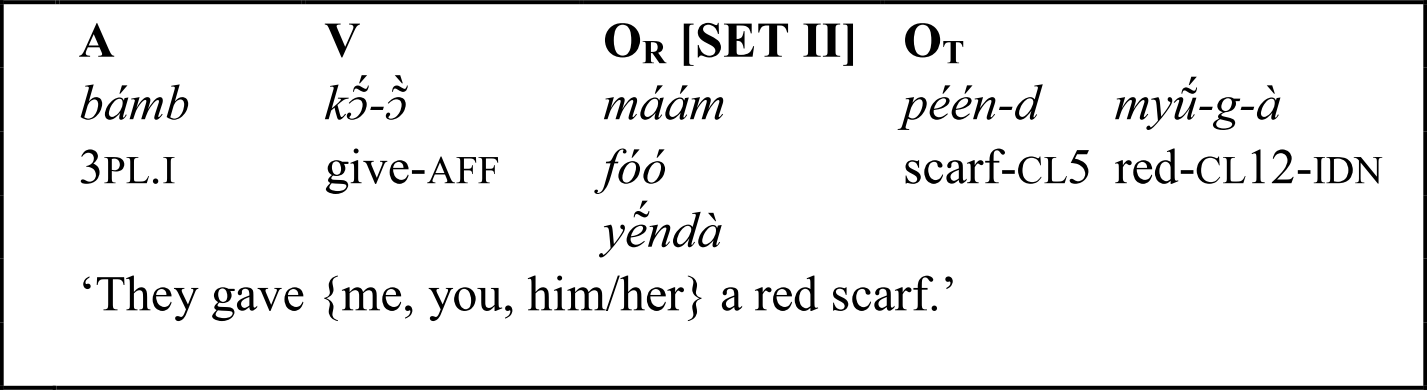
\includegraphics[width=\textwidth]{figures/pacchiarottifig1}
\caption{Set II singular forms coding the first linear object when followed by another NP}
\label{fig:1.pacchiarotti}
\end{figure}

For 1PL, 2PL and 3PL, a pronoun form from set I is used \textit{if} another NP, including one functioning as O\textsubscript{T}, an oblique, or an adverb follows (\figref{fig:2.pacchiarotti}). Using a set II pronoun form for the first linear object in \figref{fig:2.pacchiarotti} would result in ungrammaticality.

\begin{figure}[h]
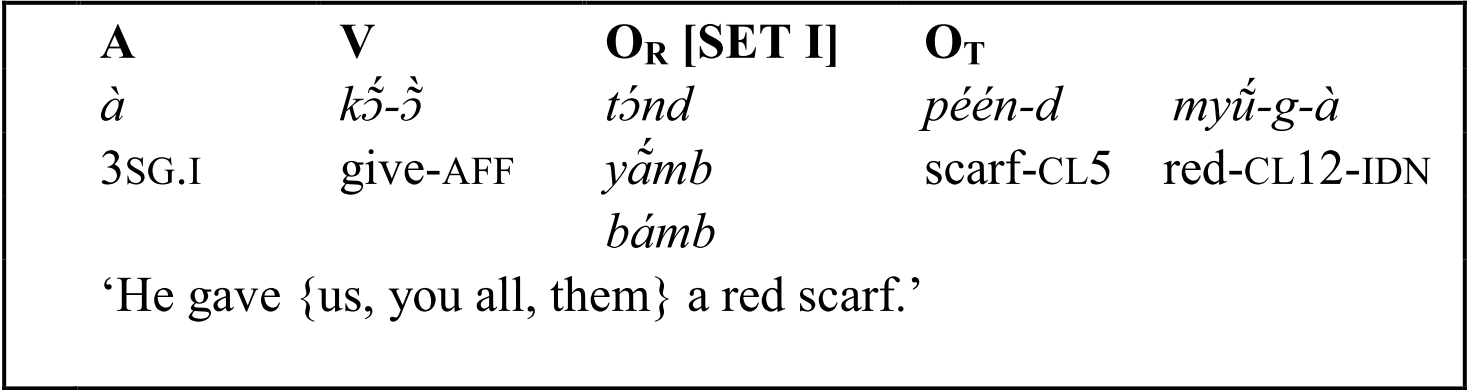
\includegraphics[width=\textwidth]{figures/pacchiarottifig2}
\caption{Set I plural forms coding the first linear object when followed by another NP}
\label{fig:2.pacchiarotti}
\end{figure}

If there is no NP following the first linear object after the verb, the plural persons are expressed by set II pronouns. This split in pronoun-form selection appears to be phonological rather than syntactic in nature (see \citealt{peterson1971} for a phonological account). This casts doubts on the nature of set II plural forms as a set of specifically case-marked `accusative' pronouns: they do not appear strictly in `object' position, but rather the set II plural forms only occur in final position within the clause. Further, while the singular persons of set I and set II differ in vowel length and tone, the plural persons of the two sets differ only in the absence vs. presence of a final vowel, respectively. 

\subsection{Optional indexation of O\textsubscript{R} and O\textsubscript{T} in relation to animacy}\label{§4.4:optional.pacchiarotti}

In Mòòré, only core syntactic object arguments can be optionally indexed\footnote{Throughout the paper, \textit{optional indexation} should be understood as a synonym of \textit{optional bound pronominal agreement}.} in the verb by the set III clitic pronouns. Obliques \ref{ex:19.pacchiarotti}, NPs followed by relator nouns like \emph{z\'{u}g\`{u}} (which in \ref{ex:21.pacchiarotti} indicates something like `off' or `from' the surface of), and locatives \ref{ex:23.pacchiarotti} cannot be indexed in the verb, as shown by the ungrammatical examples in \ref{ex:20.pacchiarotti}, \ref{ex:22.pacchiarotti} and \ref{ex:24.pacchiarotti}. 

\ea
\label{ex:19.pacchiarotti}
\gll \`{a}    M\'{u}s\'{a}    wɛ̃́-ɛ̃̀    \`{a}    R\'{i}hn\'{a}t\`{a}  nɛ́  k\'{u}g-r\`{i} \\
\textsc{3sg.i  }  M.    hit-\textsc{aff}  \textsc{3sg.i}  R.    with  stone-\textsc{cl5}\\
\glt `Musa hit Rihnata with a stone.'\footnotemark \footnotetext{Proper names are usually preceded by the 3SG pronoun\textit{ \`{a}} as shown in \ref{ex:19.pacchiarotti}. This \textit{\`{a}} is not a case marker ' it occurs before any proper name in all syntactic roles (S, A, O).}
\z

\ea[*]{
\label{ex:20.pacchiarotti}
\gll \`{a}    M\'{u}s\'{a}    wɛ̃́-ɛ̃̀-l\`{a}    \`{a}    R\'{i}hn\'{a}t\`{a} \\
\textsc{3sg.i  }  M.    hit-\textsc{3sg.iii-aff}  \textsc{3sg.i  }  R. \\
\glt (`Musa hit Rihnata with it'.)\footnotemark \footnotetext{The set III 3SG object pronoun -\textit{\`{a}} indexed in the verb in Error! Reference source not found. undergoes the same phonological process observed for the affirmative marker \textit{-\`{a}} in \sectref{§4.1:alignment.pacchiarotti}. When the shape of an immediately-preceding verb root is CV, the  set III 3SG pronoun \textit{-\`{a}} takes the form of a copy of the last vowel of the verb root, as in \ref{ex:20.pacchiarotti} where -\textit{\`{a} {\textgreater} -ɛ̃̀}{ because the verb root is CV and the last vowel is}{\textit{ ɛ̃}}{. If the contiguous verb root is not CV, then the 3SG bound pronoun surfaces as -}{\textit{\`{a}(-l\`{a})}}{ as in }{\ref{ex:22.pacchiarotti}}{ and }{\ref{ex:24.pacchiarotti}}{. (Manuel Otero, p.c.).  }}
}
\z

\ea
\label{ex:21.pacchiarotti}
\gll \`{a}    y\'{\~{e}}\'{\~{e}}s-\`{a}    z\'{i}\'{i}-m-\`{a}    f\~{u}\'{ }-g\`{\~{a}}      z\'{u}-g\`{u}\\
\textsc{3sg.i  }  wipe-\textsc{aff}  blood-\textsc{cl22-idn}  cloth-\textsc{cl12.idn}  head-\textsc{cl15}\\
\glt `She swiped the blood off the cloth.'
\z

\ea[*]{
\label{ex:22.pacchiarotti}
\gll \`{a}    y\'{\~{e}}\'{\~{e}}s-\`{a}-l\`{a}    z\'{i}\'{i}-m-\`{a} \\
\textsc{3sg.i  }  wipe-\textsc{3sg.iii-aff}  blood-\textsc{cl22-idn}\\
\glt (`She wiped the blood off it.')
}
\z

\ea
\label{ex:23.pacchiarotti}
\gll m\`{a}m    tʊ́m-\`{a}    b\'{i}\'{i}-g\`{\~{a}}      z\'{a}-k-\`{\~{e}} \\
\textsc{1sg.i  }  work-\textsc{aff}  child-\textsc{cl12.idn}  house-\textsc{cl12-loc}\\
\glt `I sent the child home.'\footnotemark \footnotetext{In Mòòré, the verb \textit{tʊ́m\`{e}} can mean `work' but also `send someone'. }
\z

\ea[*]{
\label{ex:24.pacchiarotti}
\gll m\`{a}m  tʊ́m-\`{a}-l\`{a}      b\'{i}\'{i}-g\`{\~{a}}\\
\textsc{1sg.i  }  work-\textsc{3sg.iii-aff}    child-\textsc{cl12.idn}\\
\glt (`I sent the child to it.')
}
\z

It was stated in {§4.1:alignment.pacchiarotti} that the set III bound pronouns optionally index in the verb the O of a monotransitive clause, and O\textsubscript{R} and O\textsubscript{T} of a ditransitive clause. Thus in terms of pronoun forms, Mòòré shows a neutral object alignment system in optional bound pronominal object indexation.  

In ditransitive constructions, either O\textsubscript{R} or O\textsubscript{T} can be \textit{optionally} indexed in the verb, but never both at the same time. By \textit{optionally} I mean that if either O\textsubscript{R} or O\textsubscript{T} are indexed in the verb, a lexical NP co-referential to the object that is indexed cannot occur in the clause. If one of the two objects is indexed, the other needs to be expressed either as a NP or as an independent pronoun. 

There seem to be in Mòòré no restrictions on optional bound pronominal indexation depending on a hierarchy of animacy or person (such as 1SG{\textgreater}2SG{\textgreater}3SG), plurality or definiteness. The combinations that have been tested are listed in \tabref{tab:3.pacchiarotti}.

\begin{table}
\begin{tabular}{lllll} & \textbf{O}\textbf{\textsubscript{R}} & \textbf{O}\textbf{\textsubscript{T}} & \textbf{Tested verbs} & \textbf{Indexation of O}\textbf{\textsubscript{R}}\textbf{ and O}\textbf{\textsubscript{T}}\textbf{ }\\
\lsptoprule
I & +human & +human & `show', `give' & YES\\
II & +human & +animate & `show', `send', `lend' & YES\\
III & +human & -animate & `send', `give', `tell', `teach', `ask for', `show', `leave', etc. & YES\\
IV & +animate & +animate & `show', `feed' & YES (but see below)\\
V & +animate & +human & `show' & YES\\
VI & +animate & -animate & `feed??, `show', `give' & YES\\
\lspbottomrule
\end{tabular}
\caption{Optional indexation of OR and OT depending on animacy}
\label{tab:3.pacchiarotti}

 \end{table}


For reasons of space, only combination IV is illustrated with the verb \textit{w\'{i}n\'{i}g\`{i}} `show' in \ref{ex:25.pacchiarotti}--\ref{ex:27.pacchiarotti}. Whenever both objects refer to animate or human entities, the interpretation of their semantic role is inherently ambiguous. This is true also in the case of optional indexation.

\ea
\label{ex:25.pacchiarotti}
\gll \`{a}    M\'{u}s\'{a}  w\'{i}n\'{i}g-\`{a}  b\'{a}\'{a}-g\`{\~{a}}    bʊ́ʊ́-sé \\
\textsc{3sg.i  }  M.  show-\textsc{aff}  dog-\textsc{cl12.idn}  goat-\textsc{cl13}\\
\glt `Musa showed goats to the dog.'
\z

\ea
\label{ex:26.pacchiarotti}
\gll \`{a}    M\'{u}s\'{a}  w\'{i}n\'{i}g-b-l\`{a}    b\'{a}\'{a}-g\`{\~{a}}\\
\textsc{3sg.i} M.  show-\textsc{3pl.iii-aff}  dog-\textsc{cl12.idn}\\
\glt `Musa showed them to the dog.'  
\z

\ea
\label{ex:27.pacchiarotti}
\gll \`{a}    M\'{u}s\'{a}  w\'{i}n\'{i}g-\`{a}-l\`{a}    bʊ́ʊ́-sé\\
\textsc{3sg.i  }  M.  show-\textsc{3pl.iii-aff}  goat-\textsc{cl13}\\
\glt `Musa showed goats to it (i.e. to the dog).
\z

Some verbs seem to require the indexed object to be semantically a \textsc{Recipient}, as is the case with \textit{rɪ́lg\`{e}} `feed'.\footnote{ The verb \textit{rɪ́lgé} `feed' is clearly a derived causative from the verb \textit{rɪ́} `eat', by means of the causative suffix \textit{-g}. Conceivably `show' (see \ref{ex:28.pacchiarotti}) is more lexicalized than `feed' as a ditransitive verb; perhaps there might be some restrictions on indexation of productively-derived Causees as with `feed'.} In \ref{ex:29.pacchiarotti} the indexed object corresponds to the \textsc{Recipient} of \ref{ex:28.pacchiarotti}, `lion'. The ungrammaticality of \ref{ex:30.pacchiarotti} shows that with the verb `feed'the indexed object cannot refer to the \textsc{Theme} (i.e. `sheep' in \ref{ex:28.pacchiarotti}); rather, a \textsc{Recipient} interpretation of the indexed object is forced, even if it is semantically awkward.

\ea
\label{ex:28.pacchiarotti}
\gll \`{a}    M\'{u}s\'{a}  rɪ́lg-\`{a}    bɔ̃̀yɪ́-g\`{\~{a}}    pɪ́ɪ́-s-\'{a}\\
\textsc{3sg.i  }  M.  feed-\textsc{aff}  lion-\textsc{cl12.idn}  sheep-\textsc{cl13-idn}\\
\glt `Musa fed the sheep (plural) to the lion.
\z

\ea
\label{ex:29.pacchiarotti}
\gll \`{a}    M\'{u}s\'{a}    rɪ́lg-\`{a}-l\`{a}    pɪ́ɪ́-s-\'{a}\\
\textsc{3sg.i  }  M.    feed-\textsc{3sg.iii-aff}  sheep-\textsc{cl13-idn}\\
\glt `Musa fed the sheep to it (to the lion).'
\z

\ea
\label{ex:30.pacchiarotti}
\gll \`{a}    M\'{u}s\'{a}  rɪ́lg-b-l\`{a}     bɔ̃̀yɪ́-g\`{\~{a}} \\
\textsc{3sg.i  }  M.  feed-\textsc{3pl.iii-aff  }  lion-\textsc{cl12.idn}\\
\glt
?`Musa fed the lion to them (to the sheep)' not *`Musa fed them (the sheep) to the lion.'  
\z

Examples \ref{ex:28.pacchiarotti}{}-\ref{ex:30.pacchiarotti} are the only instance I have found in which O\textsubscript{R} and O\textsubscript{T} appear to be treated differently in the language. Further research is needed to fully understand the dynamics of these `exceptions'.

\subsection{Constituency}\label{§4.5:constituency.pacchiarotti}

Adverbs of time such as `yesterday' cannot go between V and O\textsubscript{R} or between O\textsubscript{R} and O\textsubscript{T}. Thus, acceptable versions of \ref{ex:31.pacchiarotti} and \ref{ex:32.pacchiarotti} feature the temporal Adverb at the beginning or at the end of the clause, but never in a position which disrupts the sequence [V O\textsubscript{R} O\textsubscript{T}].

\ea[*]{
\label{ex:31.pacchiarotti}
\gll m\`{a}m    t\'{o}\'{o}l-\`{a}    z\'{a}\`{a}mɛ̀    p\'{a}g-\`{\~{a}}      r\'{u}-k\`{\~{a}}\\
\textsc{1sg.i  }    send-\textsc{aff}  yesterday  woman-\textsc{cl1.idn}  pot-\textsc{cl12.idn}\\
\glt (`I gave yesterday the pot to the woman.')
}
\z

\ea[*]{
\label{ex:32.pacchiarotti}
\gll m\`{a}m    t\'{o}\'{o}l-\`{a}    p\'{a}g-\`{\~{a}}      z\'{a}\`{a}mɛ̀    r\'{u}-k\`{\~{a}}\\
\textsc{1sg.i  }    send-\textsc{aff}  woman\textsc{{}-cl1.idn}  yesterday  pot-\textsc{cl12.idn}\\
\glt (`I gave to the woman yesterday the pot.')
}
\z

Identical behavior is observed with other adverbs, such as \textit{b\`{a}l\'{a}} `only' and \textit{y\`{a}s\'{a}} `again'. This indicates that the verb and its two objects form one indivisible constituent.

\section{Covert properties of ditransitive constructions}\label{§5:covert.pacchiarotti}

This section deals with covert properties of ditransitive constructions, such as controller or target of co-reference, relativization, reflexivization, etc. Passivization is excluded because in Mòòré, a functional equivalent to a passive is at most an impersonal construction in which whoever realizes an action is introduced as generic `people' and the clause construction remains transitive. Quantifier floating is irrelevant because quantifiers in Mòòré can appear only immediately after the noun they modify. 

\subsection{Relativization}\label{§5.1:relativization.pacchiarotti}

In Mòòré both O\textsubscript{R} \ref{ex:33.pacchiarotti} and O\textsubscript{T} \ref{ex:34.pacchiarotti} can be relativized by means of the same strategy:

\ea
\label{ex:33.pacchiarotti}
\gll p\'{a}g    l\'{a}nn\'{i}ng\`{a}  \'{a}    M\'{u}s\'{a}  hə̃́    t\'{o}\'{o}l  r\'{u}-k\`{\~{a}}\\
woman  \textsc{rel}    \textsc{3sg.i  }  M.  \textsc{subrd}    send  pot-\textsc{cl12.idn}\\
\glt `the woman to whom Musa sent the pot'
\z

\ea
\label{ex:34.pacchiarotti}
\gll r\'{u}-k    l\'{a}nn\'{i}ng\`{a}  \'{a}    M\'{u}s\'{a}  hə̃́    t\'{o}\'{o}l  p\'{a}g-\`{\~{a}}\\
pot-\textsc{cl12}  \textsc{rel}    \textsc{3sg.i  }  M.  \textsc{subrd}    send  woman-\textsc{cl1.idn}\\
\glt `the pot which Musa sent to the woman'
\z

In both cases, the head noun is followed by the invariable relativizer \textit{l\'{a}nn\'{i}ng\`{a}}. The relativizer is followed by the subject of the relative clause, a `subordinate' clause marker, a verb root without aspectual markers and the other object (i.e. the one that is not being relativized on). Essentially, relativization of objects occurs by means of a gap strategy. 

\subsection{Control of co-reference of possessive NPs}\label{§5.2:Control.pacchiarotti}

O\textsubscript{R} has the ability to control co-reference of a following possessor in the same way as the subject argument does.

\ea
\label{ex:35.pacchiarotti}
\gll \`{a} M\'{u}s\'{a} kɔ̃́-ɔ̃̀ \`{a} Ouérm\'{i} l\'{i}g\'{i}-d-\`{a} \textit{\`{a}} z\'{a}-k-\'{\~{o}}w\`{\~{a}}  \\
\textsc{3sg.i}  M.  give-\textsc{aff} \textsc{3sg.i} O. money-\textsc{cl21-idn} \textsc{3sg.i}  house-\textsc{cl12-loc}\\
\glt `Musa\textsubscript{i} gave the money to Ouermi\textsubscript{j} in his\textsubscript{ij} house.'
\z

When both objects are [+human], both can control co-reference of a possessor. This means that O\textsubscript{T} shows the same property as O\textsubscript{R} for the control of possessors. In \ref{ex:36.pacchiarotti}, `his house' can be the house of the subject `Musa', O\textsubscript{R} `Ouermi' or O\textsubscript{T} `the child'.

\ea
\label{ex:36.pacchiarotti}
\gll \`{a} M\'{u}s\'{a} w\'{i}n\'{i}g-\`{a} \`{a} Ouérm\'{i} b\'{i}\'{i}-g\`{\~{a}} \`{a} z\'{a}-k-\'{\~{o}}w\`{\~{a}}  \\
\textsc{3sg.i}  M.  show-\textsc{aff} \textsc{3sg.i} O. child\textsc{-cl12.idn} \textsc{3sg.i} house-\textsc{cl12-loc}\\
\glt `Musa\textsubscript{i} showed the child\textsubscript{j} to Ouermi\textsubscript{y} in his\textsubscript{ijy} house.' 
\z

\subsection{Control of co-reference under coordination and subordination}\label{§5.3:control.pacchiarotti}

In Mòòré, when a main clause has a 3SG subject and a 3SG object and a following clause has a 3SG subject, different linking elements disambiguate the possible co-reference of arguments between the two clauses. If the subject of the linearly first clause is co-referent with the subject of the second clause, the coordinator \textit{l\`{a}} is used.

\ea
\label{ex:37.pacchiarotti}
\gll \`{a}    M\'{u}s\'{a}  m\'{o}k-\`{a}    \`{a}    R\'{i}hn\'{a}t\`{a}  l\'{a}=\`{a}      l\'{o}\'{o}g-\`{e}\\
\textsc{3sg.i  }  M.  kiss-\textsc{aff}  \textsc{3sg.i} R.    and=\textsc{3sg.i  }  leave-\textsc{cfv}\\
\glt `Musa\textsubscript{i} kissed Rihnata\textsubscript{j} and he\textsubscript{i}/*she\textsubscript{j} left.' or `Musa\textsubscript{i} kissed Rihnata\textsubscript{j} and he\textsubscript{k}/she\textsubscript{k} left.'
\z

If the object of the linearly first clause if co-referential with the subject of the following clause, the complementizer \textit{tɪ́} is used:

\ea
\label{ex:38.pacchiarotti}
\gll \`{a}    M\'{u}s\'{a}  m\'{o}k-\`{a}    \`{a}    R\'{i}hn\'{a}t\`{a}  t=\`{a}        l\'{o}\'{o}g-\`{e}\\
\textsc{3sg.i  }  M.  kiss-\textsc{aff}  \textsc{3sg.i  }  R.    \textsc{compl=3sg.i  }    leave-\textsc{cfv}\\
\glt `Musa\textsubscript{i} kissed Rihnata\textsubscript{j} and *he\textsubscript{i}/she\textsubscript{j} left' or `Musa\textsubscript{i} kissed Rihnata\textsubscript{j} and he\textsubscript{k}/she\textsubscript{k} left.'
\z

When the linearly first clause is ditransitive, the same pattern described above is observed. Importantly, when \textit{tɪ́} is used, either O\textsubscript{R} or O\textsubscript{T} can be co-referential with the subject of the following clause:

\ea
\label{ex:39.pacchiarotti}
\gll \`{a}    M\'{u}s\'{a}  w\'{i}n\'{i}g-\`{a}  \`{a}    Ouérm\'{i}  b\'{i}\'{i}-g\`{\~{a}}  t=\`{a}      l\'{o}\'{o}g-\`{e} \\     
\textsc{3sg.i  }  M.  show-\textsc{aff}  \textsc{3sg.i  }  O.    child-\textsc{cl12.idn} \textsc{  compl=3sg.i}        leave-\textsc{cfv}\\
\glt `Musa\textsubscript{i}  showed the child\textsubscript{j} to Ouermi\textsubscript{y} and *he\textsubscript{i}/he\textsubscript{jk} left.'
\z

Co-reference tests were also explored under the condition of subordination \ref{ex:40.pacchiarotti}. When the subordinate clause is ditransitive and both objects are [+human], \textit{either} object can control co-reference of the subject in the main clause (along with the subject).

\ea
\label{ex:40.pacchiarotti}
\gll \`{a} M\'{u}s\'{a} hə̃̀ w\'{i}n\'{i}g \`{a} Ouérm\'{i} b\'{i}\'{i}-g\`{\~{a}} \`{a} l\'{o}\'{o}g-\`{a}-mɛ̀\\
\textsc{3sg.i  }  M.  \textsc{subrd}    show  \textsc{3sg.i  }  O.        child-\textsc{cl12.idn} \textsc{3sg.i  }  leave-\textsc{aff-phb}\\
\glt `When/since Musa\textsubscript{i} showed the child\textsubscript{j} to Ouermi\textsubscript{y} he\textsubscript{ijk} left.'
\z

Thus, in control of co-reference under coordination and subordination, as happens with control of co-reference of a possessor, O\textsubscript{R} and O\textsubscript{T} display the same behavioral properties. 

\subsection{Reflexivization and reciprocalization}\label{§5.4:reflexivization.pacchiarotti}

In Mòòré both O\textsubscript{R} \ref{ex:41.pacchiarotti} and O\textsubscript{T} \ref{ex:42.pacchiarotti} can be the target of reciprocalization:

\ea
\label{ex:41.pacchiarotti}
\gll \`{a}    Ouérm\'{i}  nɛ́  M\'{u}s\'{a}  w\'{i}n\'{i}g-\`{a}  t\'{a}\'{a}b    b\'{a}\'{a}-g\`{\~{a}} \\
\textsc{3sg.i  }  O.    with  M.  show-\textsc{aff}  each.other  dog-\textsc{cl12.idn}\\
\glt `[Musa and Ouermi]\textsubscript{i} showed the dog to each other\textsubscript{i.}'
\z

\ea
\label{ex:42.pacchiarotti}
\gll \`{a}    Ouérm\'{i}  nɛ́  M\'{u}s\'{a}  w\'{i}n\'{i}g-\`{a}  t\'{a}\'{a}b    \`{a}    Al\'{i}\\
\textsc{3sg.i    }O.    with  M.  show-\textsc{aff}  each.other  \textsc{3sg.i  }   A.\\
\glt `[Musa and Ouermi]\textsubscript{i} showed each other\textsubscript{i} to Ali.'
\z

In both cases, the reciprocal NP must immediately follow the verb, regardless of its semantic role. 

Both O\textsubscript{R }and O\textsubscript{T} can also be targets of reflexivization. In this case too, the reflexive NP must immediately follow the verb.

\ea
\label{ex:43.pacchiarotti}
\gll p\'{a}g-\`{\~{a}} kɔ̃́-ɔ̃̀ \`{a} mɛ́ng m\'{a}ng-r\`{e}\\
woman-\textsc{cl1.idn}  give-\textsc{aff}  \textsc{3sg.i  }  self  mango-\textsc{cl5}\\
\glt `The woman gave a mango to herself.'
\z

\ea
\label{ex:44.pacchiarotti}
\gll p\'{a}g-\`{\~{a}} kɔ̃́-ɔ̃̀ \`{a} mɛ́ng rà͜ò-\'{a} \\
woman-\textsc{cl1.idn}  give-\textsc{aff}  \textsc{3sg.i  }  self  man-\textsc{cl1}\\
\glt `The woman gave herself to the man.'
\z

\subsection{Information questions}\label{§5.5:Information.pacchiarotti}

In Mòòré, both O\textsubscript{R} and O\textsubscript{T} are fronted to the beginning of the clause when an information question is built upon them. 

\ea
\label{ex:45.pacchiarotti}
\gll bw\`{\~{e}}    l\'{a}    M\'{u}s\'{a}  kɔ̃́  k\'{a}m-b\`{a}?  \\
thing    which    M.  give  children-\textsc{cl1}\\
\glt `What did Musa give to the children?'
\z

\ea
\label{ex:46.pacchiarotti}
\gll \'{a}n    l\'{a}    M\'{u}s\'{a}  kɔ̃́  péén-d\`{\~{a}}? \\
person  which    M.  give  scarf-\textsc{cl5.idn}\\
\glt `To whom did Musa give the scarf?'
\z

\section{O\textsubscript{R} and O\textsubscript{T} in Mòòré ditransitive constructions within a typological perspective}\label{§6:or.pacchiarotti}

This section offers a summary of the overt and covert properties of O\textsubscript{R} and O\textsubscript{T} in Mòòré ditransitive constructions (\tabref{tab:4.pacchiarotti}), as discussed in \sectref{§4:overt.pacchiarotti} and \sectref{§5:covert.pacchiarotti}, and discusses whether double-object constructions in this language can be classified in terms of a \textsc{primary} versus \textsc{secondary object }\citep{dryer1986} type system, or \textsc{symmetrical} versus \textsc{asymmetrical} object type system \citep{bresnanmoshi1990}.

\begin{table}
\begin{tabular}{lllll} & \textbf{\textsc{object property}} & \textbf{O}\textbf{\textsubscript{R}} & \textbf{O}\textbf{\textsubscript{T}} & \textbf{Notes}\\
\lsptoprule
{ \textbf{\textsc{overt}}} & CASE MARKING & -- & -- & Neither object displays case or adpositional marking.\\
& WORD ORDER & \checkmark  & \checkmark  & Either O\textsubscript{R} and O\textsubscript{T} can appear immediately after the verb when both are [+human/animate]. \\
 & OPTIONAL BOUND PRONOMINAL AGREEMENT & \checkmark  & \checkmark  & No significant restrictions found based on animacy, number, definiteness or hierarchy of person. O\textsubscript{R} and O\textsubscript{T} cannot both be indexed at the same time.\\
 & CONSTITUENCY & \checkmark  & \checkmark  & Both appear to be a single constituent with the verb.\\
{ \textbf{\textsc{covert}}} & CONTROL OF CO-REFERENCE OF A POSSESSOR & \checkmark  & \checkmark  & Both O\textsubscript{R }and O\textsubscript{T} can control co-reference.\\
& CONTROL OF CO-REFERENCE UNDER SUBORDINATION & \checkmark  & \checkmark  & Both O\textsubscript{R }and O\textsubscript{T} can control co-reference.\\
 & RELATIVIZATION & \checkmark  & \checkmark  & The same strategy is used for O\textsubscript{R} and O\textsubscript{T}.\\
 & REFLEXIVIZATION & \checkmark  & \checkmark  & Both O\textsubscript{R }and O\textsubscript{T }can be the target.\\
 & RECIPROCALIZATION & \checkmark  & \checkmark  & Both O\textsubscript{R }and O\textsubscript{T }can be the target.\\

\lspbottomrule
\end{tabular}
\caption{Object properties in Mòòré ditransitive constructions}
\label{tab:4.pacchiarotti}

 \end{table}


Mòòré does not appear to be a \textsc{primary}/\textsc{secondary object }language in the sense of \citet{dryer1986} because both objects of a ditransitive construction display the same properties as the object of a monotransitive construction. According to \citet[147]{bresnanmoshi1991}\todo{Reference Bresnan \& Moshi 1991 is missing}, in symmetrical object languages, both objects display \textsc{primary object} properties (in the sense of \citealt{dryer1986}); the properties they test for selected Bantu languages include passivizability, object agreement, adjacency to the verb, unspecified object deletion, retention of object marking on verbs in presence of applicatives, reflexivization and reciprocalization. The authors state that in a true symmetrical object language, `different arguments can simultaneously have primary object properties' (\citealt[153]{bresnanmoshi1990}, emphasis in the original).

Many of the object properties of Bantu languages, such as passivization and object case marking, are absent in Mòòré, and the concept of `simultaneity' could pose some difficulties in the case of Mòòré just because of the morphosyntactic nature of the language itself. However, by and large this paper has shown that the two objects of a ditransitive construction in Mòòré are indistinguishable and share the same value for all the object properties that have been investigated (\tabref{tab:4.pacchiarotti}).  

\section{Conclusions}\label{§7:conclusions.pacchiarotti}

Mòòré shows a neutral object alignment system in independent pronouns and in optional bound clitic pronouns in the verb. There appears to be a split in the selection of independent pronouns for plural persons if another NP or adverb follows. This, however, should probably be considered a phonological rather than a syntactic split. Word order of objects in ditransitive clauses is strictly [+human/+animate] followed by [-animate]. Semantic role assignment is variable when both objects are [+human/animate]. In bound pronominal agreement, both O\textsubscript{R} and O\textsubscript{T} can optionally be expressed by means of bound pronouns in the verb, but never at the same time. As for constituency, both O\textsubscript{R} and O\textsubscript{T} form a constituent with the preceding verb. 

As for covert properties, O\textsubscript{R} and O\textsubscript{T} show the same relativization strategy, both can be the target of reflexivization and reciprocalization, both can control co-reference of a following possessor and co-reference under coordination/subordination. In information questions, the question word referring to both objects is fronted at the beginning of the clause. 

Based on this evidence, Mòòré appears to be a symmetrical object language type. So far, symmetrical object systems have been attested, among others, in Bantu (Bresnan \& Moshi 1990), Austronesian \citep{donohue1996}, Yagua, an isolate from Peru \citep{paynepayne1989}, Western Australian \citep{dench1995} and Totonac-Tepehua \citep{mckaytrechsel2008} languages. However, \citeauthor{bresnanmoshi1990}'s (1990)  condition of simultaneity as pivotal to defining the symmetrical object language type is not always applicable in Mòòré simply due to morphosyntactic restrictions in its grammar (e.g. only one object can be marked on the verb at a time). This suggests room for further typological research on subtypes of symmetrical object systems. It should also be noted in this respect that some of the covert properties discussed here for Mòòré are not listed among the common tests for investigating types of object systems in the literature on other languages. This raises the theoretical question of whether overt and covert properties should be assigned the same amount of `weight' or `relevance' in establishing subtypes of systems. The analysis advanced here for Mòòré also invites future comparative work on object properties in other Gur languages. This would improve the understanding of the grammatical relations in this language family and add to the typological understanding of symmetrical vs asymmetrical object systems.

\section*{Acknowledgments}

This paper would not exist without the patience of the Mòòré native speaker Timbwaoga Aimé Judicaël Ouermi, the guidance and expertise of my advisor Professor Doris L. Payne, and the stimulating comments, critiques and corrections of my friend, colleague and Africanist Manuel A. Otero. 

\section*{Abbreviations}


1  first person

2  second person

3  third person

\textsc{i} set I pronoun

\textsc{ii} set II pronoun

\textsc{iii} set III pronoun

\textsc{aff}  affirmative marker

\textsc{cfv}  citation form vowel

\textsc{cl} noun class marker

\textsc{loc} locative case marker

\textsc{idn} identifiable

\textsc{phb} (verb) phrase boundary

\textsc{pl} plural

\textsc{pvc} pre-verbal conjunction

\textsc{sg} singular



{\sloppy
\printbibliography[heading=subbibliography,notkeyword=this]
}
\end{document}